% ============================================================
%  DNS / DNSS Bayesiano con Gibbs Sampler  (v2 — tau dinamico)
%  Documentacion tecnica — Proyecto KJM
%  Compilar con: xelatex -shell-escape DNS_DNSS_Bayesiano_v2.tex
% ============================================================
\documentclass[12pt, a4paper]{article}

% ── Fuentes (XeLaTeX) ────────────────────────────────────────
\usepackage{fontspec}
\setmainfont{Latin Modern Roman}
\setsansfont{Latin Modern Sans}
\setmonofont[Scale=0.88]{Latin Modern Mono}
\usepackage{microtype}

% ── Geometria ────────────────────────────────────────────────
\usepackage[
  top=2.5cm, bottom=2.8cm,
  left=2.8cm, right=2.8cm,
  headheight=25pt
]{geometry}

% ── Colores ──────────────────────────────────────────────────
\usepackage[dvipsnames, table]{xcolor}
\definecolor{azulprincipal}{HTML}{1A3A5C}
\definecolor{azulmedio}{HTML}{2E6DA4}
\definecolor{azulclaro}{HTML}{D6E8F7}
\definecolor{azulmuyclaro}{HTML}{EEF5FC}
\definecolor{verdecod}{HTML}{1B6B3A}
\definecolor{grisclaro}{HTML}{F4F4F4}
\definecolor{grismedio}{HTML}{CCCCCC}
\definecolor{rojoacento}{HTML}{C0392B}
\definecolor{naranjacita}{HTML}{D35400}
\definecolor{verdetip}{HTML}{1E8449}

% ── Matematicas ──────────────────────────────────────────────
\usepackage{amsmath, amssymb, amsthm, mathtools}
\usepackage{bm}

% ── Tablas ───────────────────────────────────────────────────
\usepackage{booktabs}
\usepackage{tabularx}
\usepackage{multirow}
\usepackage{array}
\usepackage{longtable}
\newcolumntype{L}[1]{>{\raggedright\arraybackslash}p{#1}}
\newcolumntype{C}[1]{>{\centering\arraybackslash}p{#1}}
\newcolumntype{R}[1]{>{\raggedleft\arraybackslash}p{#1}}

% ── Graficos y TikZ ──────────────────────────────────────────
\usepackage{tikz}
\usepackage{pgfplots}
\pgfplotsset{compat=1.18}
\usetikzlibrary{arrows.meta, shapes.geometric, positioning,
                fit, backgrounds, decorations.pathreplacing, calc}

% ── Codigo fuente ────────────────────────────────────────────
\usepackage{listings}
\lstset{
  language=Python,
  basicstyle=\small\ttfamily,
  keywordstyle=\color{azulmedio}\bfseries,
  stringstyle=\color{rojoacento},
  commentstyle=\color{verdecod}\itshape,
  numberstyle=\tiny\color{gray},
  numbers=left,
  numbersep=8pt,
  breaklines=true,
  backgroundcolor=\color{grisclaro},
  showstringspaces=false,
  tabsize=4,
  frame=none,
  xleftmargin=14pt,
  framexleftmargin=14pt,
  aboveskip=4pt,
  belowskip=4pt,
  morekeywords={True,False,None,np,pd,plt,def,return,
                import,from,as,for,in,if,elif,else},
}

% ── Cajas decorativas (tcolorbox) ────────────────────────────
\usepackage[most]{tcolorbox}
\tcbuselibrary{listings, breakable, skins}

\newtcolorbox{teoremabox}[2][]{
  enhanced, breakable,
  colback=azulmuyclaro, colframe=azulmedio,
  colbacktitle=azulprincipal, coltitle=white,
  fonttitle=\bfseries\small,
  title={#2},
  sharp corners=south,
  left=6pt, right=6pt, top=4pt, bottom=4pt,
  #1
}

\newtcolorbox{notabox}[1][Nota]{
  enhanced, breakable,
  colback=grisclaro, colframe=grismedio,
  colbacktitle=grismedio, coltitle=black,
  fonttitle=\bfseries\footnotesize,
  title={#1},
  left=6pt, right=6pt, top=3pt, bottom=3pt,
  sharp corners,
}

\newtcolorbox{tipbox}[1][Recomendacion]{
  enhanced, breakable,
  colback=white, colframe=verdetip,
  borderline west={3pt}{0pt}{verdetip},
  fonttitle=\bfseries\footnotesize,
  title={#1},
  left=8pt, right=6pt, top=3pt, bottom=3pt,
  sharp corners,
  boxrule=0.4pt,
}

\newtcblisting{codigocaja}[2][]{
  enhanced, breakable,
  colback=grisclaro, colframe=azulmedio,
  colbacktitle=azulmedio!85!black, coltitle=white,
  fonttitle=\ttfamily\small,
  title={#2},
  listing only,
  listing options={
    language=Python,
    basicstyle=\small\ttfamily,
    keywordstyle=\color{azulmedio}\bfseries,
    stringstyle=\color{rojoacento},
    commentstyle=\color{verdecod}\itshape,
    numberstyle=\tiny\color{gray},
    numbers=left, numbersep=6pt,
    breaklines=true,
    showstringspaces=false,
    tabsize=4,
    morekeywords={True,False,None,np,pd,plt,def,return,
                  import,from,as,for,in,if,elif,else},
  },
  left=2pt, right=2pt, top=2pt, bottom=2pt,
  #1
}

% ── Encabezados ──────────────────────────────────────────────
\usepackage{fancyhdr}
\pagestyle{fancy}
\fancyhf{}
\fancyhead[L]{\small\color{azulmedio}\textit{DNS/DNSS Bayesiano v2 — Gibbs Sampler}}
\fancyhead[R]{\small\color{azulmedio}\textit{Proyecto KJM}}
\fancyfoot[C]{\small\color{grismedio}\thepage}
\renewcommand{\headrulewidth}{0.4pt}
\renewcommand{\headrule}{%
  \hbox to\headwidth{\color{azulmedio}\leaders\hrule height \headrulewidth\hfill}}

% ── Hipervinculos ────────────────────────────────────────────
\usepackage[
  colorlinks=true,
  linkcolor=azulmedio,
  citecolor=naranjacita,
  urlcolor=azulmedio,
  bookmarks=true,
  bookmarksnumbered=true,
]{hyperref}

% ── Secciones ────────────────────────────────────────────────
\usepackage{titlesec}
\titleformat{\section}
  {\Large\bfseries\color{azulprincipal}}
  {\thesection.}{0.8em}{}
  [\color{azulmedio}\rule{\textwidth}{0.6pt}\vspace{2pt}]

\titleformat{\subsection}
  {\large\bfseries\color{azulmedio}}
  {\thesubsection.}{0.7em}{}

\titleformat{\subsubsection}
  {\normalsize\bfseries\color{azulprincipal!70!black}}
  {\thesubsubsection.}{0.6em}{}

% ── Entornos matematicos ─────────────────────────────────────
\theoremstyle{plain}
\newtheorem{proposicion}{Proposicion}[section]
\theoremstyle{definition}
\newtheorem{definicion}{Definicion}[section]
\newtheorem{algoritmo}{Algoritmo}[section]
\theoremstyle{remark}
\newtheorem{observacion}{Observacion}[section]

% ── Macros matematicos ───────────────────────────────────────
\newcommand{\bbet}{\bm{\beta}}
\newcommand{\btau}{\bm{\tau}}
\newcommand{\bmu}{\bm{\mu}}
\newcommand{\beps}{\bm{\varepsilon}}
\newcommand{\bY}{\mathbf{Y}}
\newcommand{\by}{\mathbf{y}}
\newcommand{\bH}{\mathbf{H}}
\newcommand{\bF}{\mathbf{F}}
\newcommand{\bQ}{\mathbf{Q}}
\newcommand{\bR}{\mathbf{R}}
\newcommand{\bI}{\mathbf{I}}
\newcommand{\bP}{\mathbf{P}}
\newcommand{\bK}{\mathbf{K}}
\newcommand{\bG}{\mathbf{G}}
\newcommand{\bS}{\mathbf{S}}
\newcommand{\bzero}{\mathbf{0}}
\newcommand{\IG}{\mathcal{IG}}
\DeclareMathOperator{\N}{\mathcal{N}}
\newcommand{\TN}{\mathcal{TN}}
\newcommand{\diag}{\operatorname{diag}}
\newcommand{\tr}{\operatorname{tr}}
\newcommand{\Rhat}{\hat{R}}

% ── Miscelanea ───────────────────────────────────────────────
\usepackage{enumitem}
\usepackage{caption}
\captionsetup{font=small, labelfont={bf, color=azulprincipal}}
\usepackage{float}
\usepackage{parskip}
\setlength{\parindent}{0pt}
\setlength{\parskip}{6pt}

% ═════════════════════════════════════════════════════════════
\begin{document}
% ═════════════════════════════════════════════════════════════

% ── PORTADA ──────────────────────────────────────────────────
\begin{titlepage}
\pagecolor{azulprincipal}
\color{white}
\vspace*{1.2cm}
\begin{center}

{\small\sffamily\color{azulclaro} PROYECTO KJM --- DOCUMENTACION TECNICA --- v2}
\vspace{0.4cm}

\rule{\textwidth}{1pt}
\vspace{0.5cm}

{\Huge\bfseries\sffamily
  DNS / DNSS Bayesiano\\[0.3em]
  con Gibbs Sampler}\\[0.4em]
{\large\sffamily\color{azulclaro} \textit{Version 2 — tau dinamico}}

\vspace{0.4cm}
\rule{\textwidth}{0.4pt}
\vspace{0.5cm}

{\large\sffamily\color{azulclaro}
  Tres modos de modelado de $\tau$ - FFBS generalizado\\
  Posteriors conjugadas · MH adaptativo · Diagnosticos MCMC}

\vspace{1.8cm}

% Diagrama del ciclo Gibbs
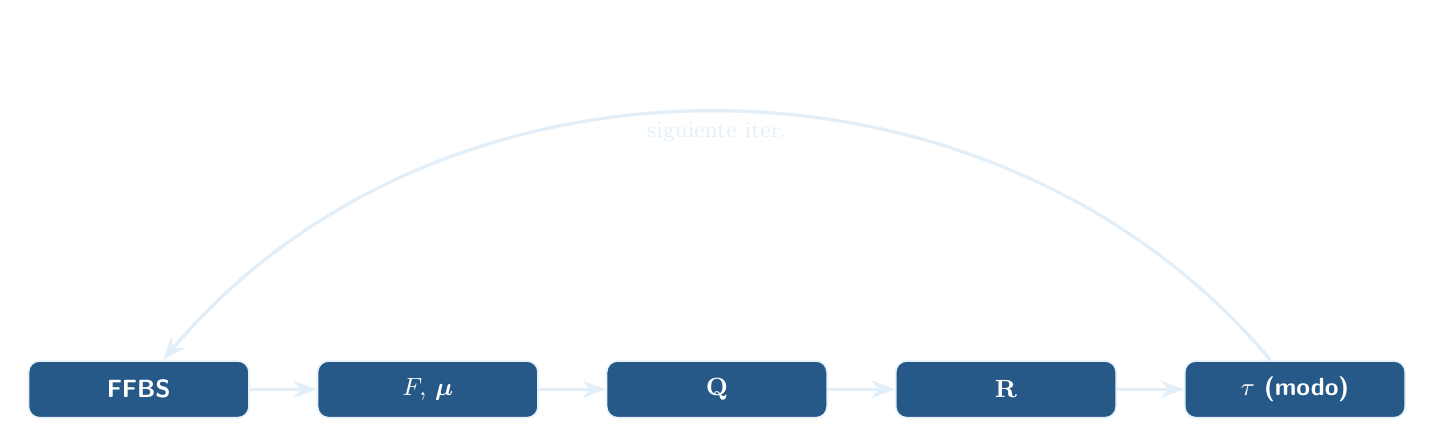
\begin{tikzpicture}[
  node distance=0.85cm,
  box/.style={
    rectangle, rounded corners=4pt,
    fill=azulmedio!60!azulprincipal,
    draw=azulclaro!60, line width=0.6pt,
    text=white, font=\small\bfseries\sffamily,
    minimum width=2.8cm, minimum height=0.72cm,
    inner sep=4pt
  },
  arr/.style={-Stealth, color=azulclaro!70, line width=1.2pt}
]
  \node[box] (ffbs)  {FFBS};
  \node[box, right=of ffbs]  (fmu) {$F,\,\bmu$};
  \node[box, right=of fmu]   (Q)   {$\bQ$};
  \node[box, right=of Q]     (R)   {$\bR$};
  \node[box, right=of R]     (tau) {$\tau$ (modo)};
  \draw[arr] (ffbs)--(fmu);
  \draw[arr] (fmu)--(Q);
  \draw[arr] (Q)--(R);
  \draw[arr] (R)--(tau);
  \draw[arr] (tau) to[bend right=50]
    node[below,font=\footnotesize\color{azulclaro!80}]{siguiente iter.} (ffbs);
\end{tikzpicture}

\vspace{1.8cm}

% Tabla de modos de tau
\begin{tabular}{ccc}
\textbf{\texttt{'estatico'}} & \textbf{\texttt{'ventana'}} & \textbf{\texttt{'ar1'}} \\[4pt]
$\tau$ global, MH & $\tau$ por ventanas & $\tau_t$ AR(1) latente \\[2pt]
Mas rapido & Semi-adaptativo & Totalmente dinamico \\
\end{tabular}

\vspace{2cm}
\rule{\textwidth}{0.4pt}
\vspace{0.4cm}

{\small\sffamily\color{azulclaro}
  Carter \& Kohn (1994) $\cdot$
  Caldeira, Laurini \& Portugal (2010) $\cdot$
  Cakmaklı (2013)\\
  Kim \& Nelson (1999) $\cdot$
  Nelson \& Siegel (1987) $\cdot$
  Svensson (1994) $\cdot$
  Gelman \& Rubin (1992)
}
\end{center}
\end{titlepage}

\nopagecolor
\color{black}

\tableofcontents
\newpage

% ═════════════════════════════════════════════════════════════
\section{Introduccion y motivacion}
% ═════════════════════════════════════════════════════════════

\subsection{Por que un enfoque bayesiano}

El estimador de Maxima Verosimilitud (MLE) con Filtro de Kalman produce
estimaciones \emph{puntuales} de los factores $\bbet_{1:T}$ y los
parametros $\bm{\theta}$. Esto tiene dos consecuencias practicas:

\begin{itemize}[leftmargin=1.5em]
  \item Los \textbf{intervalos de confianza} de los factores son condicionales
        en $\hat{\bm{\theta}}$ y subestiman la incertidumbre total.
  \item El parametro de forma $\tau$ se selecciona como un valor fijo
        (Grid Search), descartando cualquier incertidumbre sobre su valor
        y su posible variacion temporal.
\end{itemize}

El enfoque bayesiano resuelve ambos problemas al probar sobre la distribucion
posterior conjunta $p(\bbet_{1:T},\,\bm{\theta},\,\tau \mid \bY)$.

\begin{table}[H]
\centering
\caption{Comparacion Kalman Filter + MLE vs Gibbs Sampler bayesiano}
\label{tab:kf_vs_bayes}
\small
\begin{tabular}{L{3.5cm} L{5.2cm} L{5.2cm}}
\toprule
\textbf{Aspecto}
  & \textbf{Kalman Filter + MLE}
  & \textbf{Gibbs Sampler (Bayes)} \\
\midrule
Factores $\bbet_{1:T}$
  & Estimado puntual $E[\bbet_t \mid \bY, \hat{\bm{\theta}}]$
  & Distribucion completa $p(\bbet_{1:T} \mid \bY)$ \\
\addlinespace
Parametros $\bm{\theta}$
  & Optimizacion numerica (L-BFGS-B)
  & Distribucion posterior $p(\bm{\theta} \mid \bY)$ \\
\addlinespace
Incertidumbre
  & Solo la del estado ($P_{t|t}$)
  & Parametrica + de estado + de $\tau$ \\
\addlinespace
Intervalos
  & Asintóticos, condicionales en $\hat{\bm{\theta}}$
  & Intervalos de credibilidad exactos \\
\addlinespace
$\tau$
  & Fijo via Grid Search (un valor por periodo)
  & Posterior completa; opcionalmente dinamico \\
\addlinespace
Costo computacional
  & $O(T \cdot N^2 \cdot k^2)$
  & $O(n_\text{iter} \cdot T \cdot N^2 \cdot k^2)$ \\
\bottomrule
\end{tabular}
\end{table}

\subsection{Novedad de la version 2: tau dinamico}

La version 1 del notebook modelaba $\tau$ como un escalar global constante
a lo largo de toda la muestra. Esto es correcto en muestras cortas o cuando
la forma de la curva es estacionaria, pero es restrictivo cuando:

\begin{itemize}[leftmargin=1.5em]
  \item La politica monetaria cambia de regimen (e.g., TES Colombia 2019--2026).
  \item El hump de la curvatura se desplaza sistematicamente en el tiempo.
  \item El analisis cubre periodos con distintas condiciones de liquidez.
\end{itemize}

La version 2 implementa tres modos de modelado de $\tau$ seleccionables
mediante el parametro \texttt{tau\_mode} de \texttt{fit\_dns\_bayes()}.

\subsection{Estructura del notebook}

\begin{center}
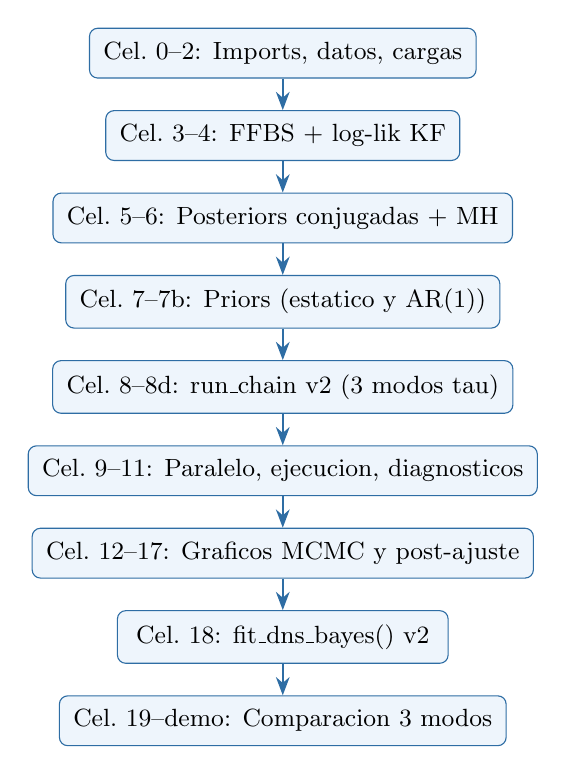
\begin{tikzpicture}[
  node distance=0.4cm and 1.5cm,
  box/.style={
    rectangle, rounded corners=3pt,
    draw=azulmedio, fill=azulmuyclaro,
    font=\small, inner sep=5pt,
    minimum width=4.2cm, minimum height=0.55cm
  },
  arr/.style={-Stealth, azulmedio, line width=0.8pt}
]
  \node[box] (c0) {Cel.\ 0--2: Imports, datos, cargas};
  \node[box, below=of c0] (c1) {Cel.\ 3--4: FFBS + log-lik KF};
  \node[box, below=of c1] (c2) {Cel.\ 5--6: Posteriors conjugadas + MH};
  \node[box, below=of c2] (c3) {Cel.\ 7--7b: Priors (estatico y AR(1))};
  \node[box, below=of c3] (c4) {Cel.\ 8--8d: run\_chain v2 (3 modos tau)};
  \node[box, below=of c4] (c5) {Cel.\ 9--11: Paralelo, ejecucion, diagnosticos};
  \node[box, below=of c5] (c6) {Cel.\ 12--17: Graficos MCMC y post-ajuste};
  \node[box, below=of c6] (c7) {Cel.\ 18: fit\_dns\_bayes() v2};
  \node[box, below=of c7] (c8) {Cel.\ 19--demo: Comparacion 3 modos};
  \foreach \a/\b in {c0/c1,c1/c2,c2/c3,c3/c4,c4/c5,c5/c6,c6/c7,c7/c8}
    \draw[arr] (\a)--(\b);
\end{tikzpicture}
\end{center}

% ═════════════════════════════════════════════════════════════
\section{Modelo espacio-estado}
% ═════════════════════════════════════════════════════════════

\subsection{Formulacion general}

\begin{teoremabox}{Modelo espacio-estado DNS/DNSS}
\textbf{Ecuacion de observacion:}
\begin{equation}
  \by_t = \bH(\btau)\,\bbet_t + \beps_t, \qquad
  \beps_t \sim \N(\bzero,\,\bR)
  \label{eq:obs}
\end{equation}
\textbf{Ecuacion de transicion:}
\begin{equation}
  \bbet_t = \bmu + \bF(\bbet_{t-1} - \bmu) + \bm{\eta}_t, \qquad
  \bm{\eta}_t \sim \N(\bzero,\,\bQ)
  \label{eq:trans}
\end{equation}
donde $\by_t \in \mathbb{R}^N$, $\bbet_t \in \mathbb{R}^k$ ($k=3$ DNS, $k=4$ DNSS),
$\bH(\btau) \in \mathbb{R}^{N \times k}$, $\bR = \diag(r_1,\ldots,r_N)$,
$\bQ = \diag(q_1,\ldots,q_k)$.
\end{teoremabox}

\subsection{\texorpdfstring{Cargas Nelson-Siegel (DNS, $k=3$)}{Cargas Nelson-Siegel (DNS, k=3)}}

\begin{equation}
  \bH_n(\tau_1) = \left[
    1,\;\;
    \frac{1-e^{-m_n/\tau_1}}{m_n/\tau_1},\;\;
    \frac{1-e^{-m_n/\tau_1}}{m_n/\tau_1} - e^{-m_n/\tau_1}
  \right]
  \label{eq:ns}
\end{equation}

El hump del factor de curvatura $\beta_{2,t}$ ocurre en
$m^* \approx 1.793\,\tau_1$ anos.

\subsection{\texorpdfstring{Cargas Nelson-Siegel-Svensson (DNSS, $k=4$)}{Cargas Nelson-Siegel-Svensson (DNSS, k=4)}}

\begin{equation}
  \bH_n(\tau_1,\tau_2) = \left[
    \bH_n(\tau_1),\;\;
    \frac{1-e^{-m_n/\tau_2}}{m_n/\tau_2} - e^{-m_n/\tau_2}
  \right]
  \label{eq:nss}
\end{equation}

Restriccion de separacion: $|\tau_1 - \tau_2| \geq 0.15$ para evitar colinealidad.

\subsection{\texorpdfstring{Estructura de $\bF$}{Estructura de F}}

\begin{table}[H]
\centering
\caption{Opciones de estructura de $\bF$}
\small
\begin{tabular}{lccc}
\toprule
\textbf{F\_type} & \textbf{Parametros en $F$} & \textbf{Muestreo} & \textbf{Referencia} \\
\midrule
\texttt{'diagonal'}   & $k$ & Normal conjugada truncada & Caldeira et al.\ (2010) P7 \\
\texttt{'triangular'} & $k(k+1)/2$ & Diagonal conj.\ + MH off-diag & Ext.\ propia \\
\texttt{'completa'}   & $k^2$ & MH matricial & VAR(1) irrestricto \\
\bottomrule
\end{tabular}
\end{table}

% ═════════════════════════════════════════════════════════════
\section{Forward Filter Backward Sampler (FFBS)}
\label{sec:ffbs}
% ═════════════════════════════════════════════════════════════

\subsection{Por que FFBS y no muestreo univariado}

Muestrear cada $\bbet_t$ condicionado en sus vecinos produce cadenas con
autocorrelacion extremadamente alta. El FFBS de Carter \& Kohn (1994)
muestrea la trayectoria \emph{completa} $\bbet_{1:T}$ en una sola pasada,
eliminando esta autocorrelacion interna.

\subsection{Algoritmo completo}

\begin{algoritmo}[FFBS --- Carter \& Kohn (1994)]
\label{alg:ffbs}
Dado $\bm{\theta} = (\bmu, \bF, \bQ, \bR, \btau)$,
muestrear $\bbet_{1:T} \sim p(\bbet_{1:T} \mid \bY, \bm{\theta})$.

\textbf{Fase forward (Kalman Filter):} para $t = 1, \ldots, T$:
\begin{align}
  \hat{\bbet}_{t|t-1} &= \bmu + \bF(\hat{\bbet}_{t-1|t-1} - \bmu) \\
  \bP_{t|t-1} &= \bF\,\bP_{t-1|t-1}\,\bF^\top + \bQ \\
  \bm{v}_t &= \by_t - \bH\,\hat{\bbet}_{t|t-1} \\
  \bS_t &= \bH\,\bP_{t|t-1}\,\bH^\top + \bR \\
  \bK_t &= \bP_{t|t-1}\,\bH^\top\,\bS_t^{-1} \\
  \hat{\bbet}_{t|t} &= \hat{\bbet}_{t|t-1} + \bK_t\,\bm{v}_t \\
  \bP_{t|t} &= (\bI - \bK_t\bH)\,\bP_{t|t-1}\,(\bI - \bK_t\bH)^\top
               + \bK_t\bR\bK_t^\top \quad \text{(forma Joseph)}
  \label{eq:joseph}
\end{align}

\textbf{Fase backward:}
muestrear $\bbet_T \sim \N(\hat{\bbet}_{T|T},\, \bP_{T|T})$.
Para $t = T-1,\ldots,1$:
\begin{align}
  \bP_{t+1|t} &= \bF\,\bP_{t|t}\,\bF^\top + \bQ \\
  \bG_t &= \bP_{t|t}\,\bF^\top\,\bP_{t+1|t}^{-1}
           \quad\text{(ganancia suavizadora)} \\
  \bm{\mu}_{t|T} &= \hat{\bbet}_{t|t}
    + \bG_t\!\left(\bbet_{t+1} - \hat{\bbet}_{t+1|t}\right) \\
  \bm{\Sigma}_{t|T} &= \bP_{t|t} - \bG_t\,\bP_{t+1|t}\,\bG_t^\top \\
  \bbet_t &\sim \N\!\left(\bm{\mu}_{t|T},\;\bm{\Sigma}_{t|T}\right)
\end{align}
\end{algoritmo}

\begin{notabox}[Forma Joseph (ecuacion~\ref{eq:joseph})]
La actualizacion de $\bP_{t|t}$ usa la forma Joseph
$(I-KH)P(I-KH)^\top + KRK^\top$
en lugar de la forma estandar $(I-KH)P$.
Garantiza simetria y positividad definida ante errores de redondeo acumulados.
\end{notabox}

\subsection{Inicializacion estacionaria}

Para $\bF$ diagonal, la condicion inicial $\bP_{0|0}$ se obtiene directamente:
\begin{equation}
  P_{0,ii} = \frac{q_i}{1 - f_i^2}, \qquad i = 1,\ldots,k
  \label{eq:lyapunov}
\end{equation}

\subsection{Implementacion}

La funcion \texttt{\_ffbs\_diag()} esta compilada con Numba JIT para F diagonal
y es valida para $k=3$ (DNS) y $k=4$ (DNSS) sin modificar el codigo.
El wrapper publico \texttt{ffbs()} garantiza los tipos correctos:

\begin{codigocaja}{Celda 3 --- ffbs() (wrapper publico)}
def ffbs(mu, f_vec, q_vec, r_vec, H, yields):
    '''Wrapper FFBS para F diagonal. Valido k=3 (DNS) y k=4 (DNSS).'''
    return _ffbs_diag(
        np.asarray(mu,     dtype=np.float64),
        np.asarray(f_vec,  dtype=np.float64),  # diag(F): (k,)
        np.asarray(q_vec,  dtype=np.float64),  # diag(Q): (k,)
        np.asarray(r_vec,  dtype=np.float64),  # diag(R): (N,)
        np.asarray(H,      dtype=np.float64),  # cargas:  (N, k)
        np.asarray(yields, dtype=np.float64),  # datos:   (T, N)
    )
    # Retorna: betas (T, k) --- una trayectoria de la posterior
\end{codigocaja}

% ═════════════════════════════════════════════════════════════
\section{Distribuciones posteriores conjugadas}
% ═════════════════════════════════════════════════════════════

Condicionado en $\bbet_{1:T}$ (muestreado por FFBS), todos los demas
parametros tienen posteriors analiticas exactas.

\subsection{\texorpdfstring{Posterior de $\bmu$ y $f_i$ (Normal conjugada)}{Posterior de mu y f_i (Normal conjugada)}}

\begin{teoremabox}{Posterior de $\mu_i$ dado $f_i$}
Con prior $\mu_i \sim \N(m_{0i},\, V_{0i})$,
definiendo $\ell_{i,t} = \beta_{i,t} - f_i\,\beta_{i,t-1}$:
\begin{equation}
  \mu_i \mid f_i, \bbet, q_i \;\sim\; \N\!\left(\bar{m}_i,\; \bar{V}_i\right)
\end{equation}
\begin{equation}
  \bar{V}_i^{-1} = \frac{1}{V_{0i}} + \frac{(1-f_i)^2\,T_\text{eff}}{q_i},
  \qquad
  \bar{m}_i = \bar{V}_i\!\left(
    \frac{m_{0i}}{V_{0i}} + \frac{1-f_i}{q_i}\sum_t \ell_{i,t}
  \right)
  \label{eq:post_mu}
\end{equation}
donde $T_\text{eff} = T-1$.
\end{teoremabox}

\begin{teoremabox}{Posterior de $f_i$ dado $\mu_i$ (Normal truncada)}
Definiendo $a_{i,t} = \beta_{i,t} - \mu_i$:
\begin{equation}
  f_i \mid \mu_i, \bbet, q_i \;\sim\;
  \TN_{(-1,1)}\!\left(\bar{f}_i,\;\bar{V}_{f_i}\right)
\end{equation}
\begin{equation}
  \bar{V}_{f_i}^{-1} = \frac{1}{V_{f_{0i}}} + \frac{\sum_t a_{i,t-1}^2}{q_i},
  \qquad
  \bar{f}_i = \bar{V}_{f_i}\!\left(
    \frac{f_{0i}}{V_{f_{0i}}} + \frac{\sum_t a_{i,t}\,a_{i,t-1}}{q_i}
  \right)
  \label{eq:post_f}
\end{equation}
La truncacion en $(-1,1)$ garantiza estacionariedad del AR(1) de cada factor.
\end{teoremabox}

\begin{observacion}
El muestreo es secuencial: $\mu_i \to f_i$ por cada factor $i = 1,\ldots,k$.
Esto es Gibbs dentro de Gibbs y garantiza consistencia interna en cada iteracion.
\end{observacion}

\subsection{Posterior de $q_i$ (Inverse-Gamma conjugada)}

Con residuos de estado $\eta_{i,t} = \beta_{i,t} - \mu_i - f_i(\beta_{i,t-1}-\mu_i)$:

\begin{equation}
  q_i \mid \bbet, \mu_i, f_i \;\sim\;
  \IG\!\left(a_0 + \frac{T_\text{eff}}{2},\;\;
    b_0 + \frac{\sum_t \eta_{i,t}^2}{2}\right)
  \label{eq:post_q}
\end{equation}

\subsection{Posterior de $r_n$ (Inverse-Gamma conjugada)}

Con residuos de medicion $\varepsilon_{n,t} = y_{t,n} - \bH_n\,\bbet_t$:

\begin{equation}
  r_n \mid \bbet, \bY \;\sim\;
  \IG\!\left(a_0 + \frac{T}{2},\;\;
    b_0 + \frac{\sum_t \varepsilon_{n,t}^2}{2}\right)
  \label{eq:post_r}
\end{equation}

\subsection{Extensiones para plazos largos}

\subsubsection{Opcion A --- $\bR$ estructurada por grupos de plazos}

En lugar de estimar $N$ varianzas independientes, se reducen a 3 parametros
por grupos de plazos (corto $\leq$ th1, medio $\leq$ th2, largo $>$ th2).
La posterior por grupo $\mathcal{G}_g$ recoge todos sus residuos:

\begin{equation}
  r_g \mid \bbet, \bY \;\sim\;
  \IG\!\left(a_0 + \frac{T\,|\mathcal{G}_g|}{2},\;\;
    b_0 + \frac{\sum_{n \in \mathcal{G}_g}\sum_t \varepsilon_{n,t}^2}{2}\right)
  \label{eq:post_r_grupos}
\end{equation}

\subsubsection{Opcion C --- Pesos en la posterior de $\bR$}

Asignar peso $w_n > 1$ a un plazo $n$ reduce el $b_0$ efectivo,
concentrando la posterior en valores menores de $r_n$ (mejor ajuste):

\begin{equation}
  r_n^{(w)} \mid \bbet, \bY \;\sim\;
  \IG\!\left(a_0 + \frac{T}{2},\;\;
    \frac{b_0}{w_n} + \frac{\sum_t \varepsilon_{n,t}^2}{2}\right)
  \label{eq:post_r_pesos}
\end{equation}

% ═════════════════════════════════════════════════════════════
\section{Metropolis-Hastings para $\tau$ --- modo estatico}
\label{sec:mh_estatico}
% ═════════════════════════════════════════════════════════════

\subsection{Log-verosimilitud marginal}

$\tau$ entra de forma no lineal en $\bH(\tau)$, por lo que no existe familia
conjugada. Se usa MH con la log-verosimilitud \emph{marginal}
$p(\bY \mid \tau, \bm{\theta})$ donde $\bbet_{1:T}$ esta integrado via KF:

\begin{equation}
  \log p(\bY \mid \tau, \bm{\theta}) =
  -\frac{TN}{2}\log(2\pi)
  -\frac{1}{2}\sum_{t=1}^T \bigl[\log|\bS_t| + \bm{v}_t^\top \bS_t^{-1} \bm{v}_t\bigr]
  \label{eq:marglik}
\end{equation}

El $\log|\bS_t|$ se calcula via Cholesky para estabilidad numerica.

\begin{notabox}[Por que log-verosimilitud marginal y no condicional en $\bbet$]
Si se evaluara la log-lik con la trayectoria $\bbet_{1:T}$ del paso anterior
(que fue muestreada con el $\tau$ antiguo), la comparacion seria inconsistente:
$\bbet$ y $\tau^*$ usarian parametros de forma distintos.
La log-lik marginal promedia correctamente sobre todas las trayectorias
posibles, garantizando que el ratio de aceptacion sea valido.
\end{notabox}

\subsection{Propuesta y ratio de aceptacion}

\begin{teoremabox}{MH para $\tau$ --- propuesta random walk en log-escala}
Para garantizar positividad sin truncar el espacio:
\begin{align}
  \text{DNS:}  &\quad \log\tau_1^* = \log\tau_1 + \sigma_1\,z,
                \quad z \sim \N(0,1) \\
  \text{DNSS:} &\quad \begin{pmatrix}\log\tau_1^*\\\log\tau_2^*\end{pmatrix}
                = \begin{pmatrix}\log\tau_1\\\log\tau_2\end{pmatrix}
                + \begin{pmatrix}\sigma_1 z_1\\\sigma_2 z_2\end{pmatrix},
                \quad z_1,z_2 \overset{iid}{\sim} \N(0,1)
\end{align}
Ratio de aceptacion ($\alpha = \min(1,\,e^{\log\alpha})$):
\begin{equation}
  \log\alpha =
  \underbrace{
    \log p(\bY \mid \tau^*, \bm{\theta}) - \log p(\bY \mid \tau, \bm{\theta})
  }_{\Delta\text{log-lik}}
  +
  \underbrace{
    \log p(\tau^*) - \log p(\tau)
  }_{\Delta\text{log-prior}}
  \label{eq:mh_ratio}
\end{equation}
El Jacobiano del cambio de variables $\log\tau \to \tau$ cancela porque la
propuesta es simetrica en log-escala.
\end{teoremabox}

\subsection{Adaptacion durante el burn-in}

La std de la propuesta $\sigma$ se ajusta cada $n_\text{burnin}/5$ iteraciones:
\begin{equation}
  \sigma \leftarrow
  \begin{cases}
    0.70\,\sigma & \text{si } \hat{r} < r_\text{target} - 0.12 \\
    1.35\,\sigma & \text{si } \hat{r} > r_\text{target} + 0.15 \\
    \sigma       & \text{en otro caso}
  \end{cases}
  \label{eq:adapt}
\end{equation}
con $r_\text{target} = 0.40$ (DNS, 1D) y $r_\text{target} = 0.28$ (DNSS, 2D),
y $\sigma$ acotado en $[0.005,\, 0.60]$.

% ═════════════════════════════════════════════════════════════
\section{Modos de modelado de $\tau$ (novedad v2)}
\label{sec:tau_modos}
% ═════════════════════════════════════════════════════════════

La version 2 permite elegir entre tres modos de modelado de $\tau$
mediante el parametro \texttt{tau\_mode}. El modo \texttt{'estatico'}
(Seccion~\ref{sec:mh_estatico}) es el comportamiento clasico de la v1.
Los modos \texttt{'ventana'} y \texttt{'ar1'} permiten capturar variacion
temporal de la forma de la curva.

\begin{table}[H]
\centering
\caption{Comparativa de los tres modos de tau}
\label{tab:tau_modos}
\small
\begin{tabular}{L{2.2cm} L{4.5cm} L{4.0cm} L{3.0cm}}
\toprule
\textbf{Modo} & \textbf{Descripcion} & \textbf{Ventajas} & \textbf{Limitaciones} \\
\midrule
\texttt{'estatico'} &
  $\tau$ global unico para toda la muestra. Posterior via MH estandar. &
  Mas rapido; IC de $\tau$ bien definido; minimo de parametros. &
  Asume forma de curva constante en $t$. \\
\addlinespace
\texttt{'ventana'} &
  $\tau$ cambia entre ventanas rodantes de tamano $W$. Mini-sampler por ventana. &
  Semi-adaptativo sin cambio de modelo; facil de interpretar. &
  IC de $\tau$ mas amplios por menor informacion en cada ventana. \\
\addlinespace
\texttt{'ar1'} &
  $\tau_t$ sigue AR(1) latente en log-escala con hiperparametros $\phi_x$, $\sigma_x$. &
  Totalmente dinamico; captura cambios de regimen de forma continua. &
  El mas lento; requiere mas iteraciones para convergencia. \\
\bottomrule
\end{tabular}
\end{table}

\subsection{Modo \texttt{'ventana'} --- $\tau$ semi-adaptativo}

La muestra se divide en ventanas solapadas de tamano $W$
con desplazamiento $s$:
\begin{equation}
  \mathcal{W}_j = [j\cdot s,\;\; j\cdot s + W - 1], \qquad
  j = 0, 1, \ldots, \left\lfloor\frac{T - W}{s}\right\rfloor
  \label{eq:ventana}
\end{equation}

En cada ventana se corre un mini-sampler de 5 pasos de MH con la
log-lik local $p(\bY_{\mathcal{W}_j} \mid \tau, \bm{\theta})$.
La secuencia temporal $\tau_t$ se ensambla promediando las estimaciones
de todas las ventanas que contienen el periodo $t$.

\begin{tipbox}[Eleccion de $W$]
Para datos mensuales de TES Colombia, se recomienda $W \approx 36$--$60$ meses
(3--5 anos). Ventanas mas grandes producen $\tau_t$ mas suaves; ventanas
menores capturan cambios mas rapidos pero con mayor varianza.
\end{tipbox}

\subsection{Modo \texttt{'ar1'} --- $\tau_t$ latente con dinamica AR(1)}

\subsubsection{Especificacion del proceso}

Se define $x_t = \log\tau_{1,t}$ (y $z_t = \log\tau_{2,t}$ para DNSS)
como proceso AR(1) latente en log-escala:
\begin{equation}
  x_t = \mu_x + \phi_x(x_{t-1} - \mu_x) + \sigma_x\,\varepsilon_t, \qquad
  \varepsilon_t \sim \N(0, 1)
  \label{eq:tau_ar1}
\end{equation}

La log-escala garantiza $\tau_t = e^{x_t} > 0$ en todo momento.
La media $\mu_x = \log(\tau_\text{init})$ se fija en la inicializacion OLS.

\subsubsection{Priors sobre los hiperparametros}

\begin{equation}
  \phi_x \sim \TN_{(0,1)}\!\left(0.95,\; 0.05^2\right)
  \label{eq:prior_phi_x}
\end{equation}
\begin{equation}
  \sigma_x^2 \sim \IG\!\left(2,\; 0.01\right)
  \label{eq:prior_sigma_x}
\end{equation}

El prior de $\phi_x$ centrado en 0.95 refleja que $\tau_t$ cambia lentamente
(alta persistencia). El prior de $\sigma_x^2$ muy pequeno evita cambios abruptos.

\subsubsection{Muestreo de $x_{1:T}$ via MH por periodo}

Para cada $t = 1,\ldots,T$, se propone $x_t^* = x_t + \sigma_\text{prop}\,z$
y se acepta con ratio:
\begin{equation}
  \log\alpha_t =
  \underbrace{
    \log p(\by_t \mid x_t^*, \bbet_t, \bR)
    - \log p(\by_t \mid x_t,  \bbet_t, \bR)
  }_{\Delta\text{log-lik local}}
  +
  \underbrace{
    \log p(x_t^* \mid x_{t-1}, x_{t+1})
    - \log p(x_t  \mid x_{t-1}, x_{t+1})
  }_{\Delta\text{log-prior condicional}}
  \label{eq:mh_ar1}
\end{equation}

La log-lik local para el periodo $t$ es:
\begin{equation}
  \log p(\by_t \mid x_t, \bbet_t, \bR) =
  -\frac{1}{2}\sum_{n=1}^N \left[
    \frac{(y_{t,n} - \bH_n(e^{x_t})\,\bbet_t)^2}{r_n}
    + \log(2\pi r_n)
  \right]
  \label{eq:loglik_local}
\end{equation}

La prior condicional de $x_t$ dado sus vecinos es:
\begin{equation}
  \log p(x_t \mid x_{t-1}, x_{t+1}) \propto
  -\frac{1}{2\sigma_x^2}\!\left[
    \bigl(x_t - \mu_x - \phi_x(x_{t-1}-\mu_x)\bigr)^2 +
    \bigl(x_{t+1} - \mu_x - \phi_x(x_t - \mu_x)\bigr)^2
  \right]
  \label{eq:ar1_cond}
\end{equation}

\subsubsection{Posteriors conjugadas de los hiperparametros}

\begin{teoremabox}{Posterior de $\phi_x$ dado $x_{1:T}$}
Con $a_t = x_t - \mu_x$ y prior $\phi_x \sim \TN_{(0,1)}(\bar{\phi}, V_\phi)$:
\begin{equation}
  \phi_x \mid x_{1:T}, \sigma_x \;\sim\;
  \TN_{(0,1)}\!\left(
    \frac{\bar{\phi}/V_\phi + \sum_t a_{t-1}a_t/\sigma_x^2}
         {1/V_\phi + \sum_t a_{t-1}^2/\sigma_x^2},\;\;
    \left[\frac{1}{V_\phi} + \frac{\sum_t a_{t-1}^2}{\sigma_x^2}\right]^{-1}
  \right)
  \label{eq:post_phi_x}
\end{equation}
\end{teoremabox}

\begin{teoremabox}{Posterior de $\sigma_x^2$ dado $x_{1:T}$}
Con residuos $\eta_t = x_t - \mu_x - \phi_x(x_{t-1}-\mu_x)$:
\begin{equation}
  \sigma_x^2 \mid x_{1:T}, \phi_x \;\sim\;
  \IG\!\left(a_0 + \frac{T-1}{2},\;\;
    b_0 + \frac{\sum_{t=2}^T \eta_t^2}{2}\right)
  \label{eq:post_sigma_x}
\end{equation}
\end{teoremabox}

\subsubsection{Ciclo Gibbs completo con modo AR(1)}

\begin{algoritmo}[Gibbs con $\tau_t$ AR(1)]
\label{alg:gibbs_ar1}
Por cada iteracion $s$:
\begin{enumerate}[leftmargin=1.5em, itemsep=2pt]
  \item $\bbet_{1:T} \mid \bar{\tau}, \bm{\theta}$
    $\to$ \textbf{FFBS} con $\bH(\bar{\tau})$,
    donde $\bar{\tau} = \operatorname{mediana}(e^{x_{1:T}})$
  \item $\bF, \bmu \mid \bbet, \bQ$
    $\to$ Normal conjugada truncada (diagonal)
  \item $\bQ \mid \bbet, \bF, \bmu$
    $\to$ Inverse-Gamma conjugada
  \item $\bR \mid \bbet, \bY$
    $\to$ IG conjugada (libre, grupos, o ponderada)
  \item $x_{1:T} \mid \bbet, \bm{\theta}, \phi_x, \sigma_x$
    $\to$ MH por periodo (ec.~\ref{eq:mh_ar1})
  \item $\phi_x \mid x_{1:T}, \sigma_x$
    $\to$ Normal truncada conjugada (ec.~\ref{eq:post_phi_x})
  \item $\sigma_x^2 \mid x_{1:T}, \phi_x$
    $\to$ Inverse-Gamma conjugada (ec.~\ref{eq:post_sigma_x})
\end{enumerate}
\end{algoritmo}

\begin{tipbox}[Calibracion de tau\_ar1\_prop\_std]
La std de propuesta por periodo \texttt{tau\_ar1\_prop\_std} controla la
tasa de aceptacion del MH local. Se recomienda comenzar con 0.04--0.06
y ajustar para obtener una tasa media entre 30\% y 55\%.
Una tasa muy alta indica que $\tau_t$ varia poco y el modo \texttt{'estatico'}
puede ser suficiente.
\end{tipbox}

% ═════════════════════════════════════════════════════════════
\section{Especificacion de priors}
% ═════════════════════════════════════════════════════════════

Los priors siguen la filosofia debilmente informativos de
Caldeira et al.\ (2010) y Cakmaklı (2013).

\begin{table}[H]
\centering
\caption{Especificacion de priors --- funcion \texttt{make\_priors()}}
\label{tab:priors}
\small
\begin{tabular}{L{3.5cm} L{4cm} L{6.5cm}}
\toprule
\textbf{Parametro} & \textbf{Prior} & \textbf{Justificacion} \\
\midrule
$f_i$
  & $\TN_{(-1,1)}(0.90,\,0.10^2)$
  & Alta persistencia tipica en DNS; truncacion garantiza estacionariedad \\
\addlinespace
$\mu_i$
  & $\N(m_{0i},\,25)$
  & Difuso; centrado en valores historicos plausibles \\
\addlinespace
$q_i,\,r_n$
  & $\IG(0.01,\,0.01)$
  & Casi no-informativo (Jeffreys-like) \\
\addlinespace
$\tau$ (uniforme)
  & $\mathcal{U}(0.15,\,5.0)$
  & Bounds economicos; hump en $[0.27, 9.0]$ anos \\
\addlinespace
$\tau_1$ (normal)
  & $\N(1.78,\,0.40^2)$
  & Prior informativo; hump esperado en $\approx 3.2$ anos \\
\addlinespace
$\tau_2$ (normal)
  & $\N(0.60,\,0.08^2)$
  & Fuertemente informativo; evita colinealidad con $\tau_1$ \\
\addlinespace
$\phi_x$ (AR(1) de $\tau$)
  & $\TN_{(0,1)}(0.95,\,0.05^2)$
  & Alta persistencia de $\tau_t$; solo para \texttt{tau\_mode='ar1'} \\
\addlinespace
$\sigma_x^2$ (AR(1) de $\tau$)
  & $\IG(2,\,0.01)$
  & Varianza pequena; $\tau_t$ cambia lentamente \\
\bottomrule
\end{tabular}
\end{table}

\begin{codigocaja}{Celda 7 / 7b --- make\_priors() y make\_priors\_ar1()}
# Prior uniforme (difuso, modo estatico o ventana)
priors = make_priors('DNSS', prior_tau_type='uniforme',
                     tau_lo=0.15, tau_hi=5.0)

# Prior normal informativo (cuando se conoce el regimen)
priors = make_priors('DNSS', prior_tau_type='normal',
                     tau1_mu=1.78, tau1_sd=0.40,
                     tau2_mu=0.60, tau2_sd=0.08)

# Priors extendidos para modo AR(1)
priors = make_priors_ar1('DNS', tau1_init=1.78,
                          phi_x_mean=0.95, phi_x_sd=0.05,
                          sigma_x_a=2.0,   sigma_x_b=0.01)
\end{codigocaja}

% ═════════════════════════════════════════════════════════════
\section{Diagnosticos de convergencia MCMC}
% ═════════════════════════════════════════════════════════════

\subsection{Estadistico $\hat{R}$ de Gelman-Rubin}

\begin{teoremabox}{$\hat{R}$ de Gelman-Rubin (1992)}
Con $m$ cadenas de longitud $n$ para un parametro escalar $\psi$:
\begin{align}
  B &= \frac{n}{m-1}\sum_{j=1}^m (\bar{\psi}_j - \bar{\psi})^2 \\
  W &= \frac{1}{m}\sum_{j=1}^m s_j^2 \\
  \hat{R} &= \sqrt{\frac{(n-1)W/n + B/n}{W}}
\end{align}
\textbf{Criterios:} $\hat{R} < 1.05$ (excelente),
$\hat{R} < 1.10$ (aceptable),
$\hat{R} \geq 1.10$ (no convergio --- extender iteraciones).
\end{teoremabox}

\subsection{Effective Sample Size (ESS)}

\begin{equation}
  \text{ESS} = \frac{n}{1 + 2\sum_{k=1}^{\infty}\hat{\rho}_k}
  \label{eq:ess}
\end{equation}

La suma se trunca cuando $|\hat{\rho}_k| < 0.05$.
Se considera aceptable ESS $> 400$ y pobre ESS $< 100$.

\subsection{Visualizaciones de diagnostico}

El notebook genera tres bloques de diagnostico MCMC:

\begin{enumerate}[leftmargin=1.5em]
  \item \textbf{Traceplots} (\texttt{plot\_traceplots}):
        evolucion de los parametros por iteracion.
        Una cadena bien mezclada explora el espacio, se solapa entre cadenas
        y no tiene tendencia sistematica.
  \item \textbf{ACF de la cadena} (\texttt{plot\_acf\_mcmc}):
        funcion de autocorrelacion de las muestras con ESS por parametro.
  \item \textbf{Distribuciones posteriores} (\texttt{plot\_posteriors}):
        histogramas con KDE, media posterior e IC 95\%.
\end{enumerate}

% ═════════════════════════════════════════════════════════════
\section{Documentacion de funciones}
% ═════════════════════════════════════════════════════════════

\subsection{Cargas}

\begin{codigocaja}{Celda 2 --- cargas NS y NSS}
def ns_loadings(maturities, tau1):
    '''Nelson-Siegel. Shape (N, 3): [nivel, pendiente, curvatura].'''
    ...

def nss_loadings(maturities, tau1, tau2):
    '''Nelson-Siegel-Svensson. Shape (N, 4).
    Condicion: |tau1 - tau2| >= 0.15 para evitar colinealidad.'''
    ...

def get_H(maturities, tau1, tau2, model):
    '''Wrapper: model='DNS' -> ns_loadings | 'DNSS' -> nss_loadings.'''
    ...
\end{codigocaja}

\subsection{Posteriors conjugadas}

\begin{codigocaja}{Celda 5 --- muestreo de F, mu, Q, R}
# F diagonal y mu --- Normal conjugada
f_new, mu_new = sample_F_mu_diagonal(
    betas,                            # (T, k) trayectoria FFBS actual
    f_vec, q_vec,                     # parametros actuales
    prior_f_mean, prior_f_var,        # prior de f_i
    prior_mu_mean, prior_mu_var)      # prior de mu_i

# Q --- Inverse-Gamma por factor
q_new = sample_Q(betas, mu, f_vec, prior_Q_a, prior_Q_b)

# R --- libre: N varianzas independientes
r_new = sample_R(yields, betas, H, prior_R_a, prior_R_b,
                 obs_weights=None)    # Opcion C: pesos por plazo

# R --- grupos: 3 varianzas por tramo (Opcion A)
r_new = sample_R_groups(yields, betas, H, prior_R_a, prior_R_b,
                         maturities, group_thresholds=(3.0, 10.0))
\end{codigocaja}

\subsection{Muestreo de $\tau$}

\begin{codigocaja}{Celda 6 --- MH para tau (modo estatico)}
# DNS: MH 1D para tau1
tau1, loglik_new, accepted = sample_tau_MH_dns(
    tau1, yields, mu, f_vec, q_vec, r_vec,
    maturities,
    prop_std  = 0.08,
    tau_bounds= (0.15, 5.0),
    prior_tau = ('uniforme', 0.15, 5.0))

# DNSS: MH 2D para (tau1, tau2)
tau1, tau2, loglik_new, accepted = sample_tau_MH_dnss(
    tau1, tau2, yields, mu, f_vec, q_vec, r_vec,
    maturities,
    prop_std   = np.array([0.08, 0.06]),
    tau_bounds = (0.15, 5.0),
    prior_tau  = ('normal', 1.78, 0.40, 0.60, 0.08),
    sep_min    = 0.15)
\end{codigocaja}

\begin{codigocaja}{Celda 8b --- muestreo de tau AR(1)}
# Muestrea x_1:T = log(tau_t) via MH por periodo
x_seq, acc_rate = sample_tau_ar1_MH(
    x_seq,        # (T, n_tau) secuencia actual de log(tau_t)
    betas,        # (T, k) trayectoria FFBS actual
    yields,       # (T, N)
    r_vec,        # (N,) varianzas de medicion actuales
    model, maturities,
    phi_x,        # float o (n_tau,) persistencia AR(1)
    mu_x,         # float o (n_tau,) media de largo plazo
    sigma_x,      # float o (n_tau,) std de innovaciones
    prop_std_t=0.05)
# Retorna: x_seq actualizado (T, n_tau), acc_rate float

# Muestrea hiperparametros del proceso AR(1)
phi_x   = sample_phi_x(x_seq, mu_x, sigma_x,
                        phi_x_mean=0.95, phi_x_var=0.05**2)
sigma_x = sample_sigma_x(x_seq, mu_x, phi_x,
                          sigma_x_a=2.0, sigma_x_b=0.01)
\end{codigocaja}

\subsection{Modo ventana}

\begin{codigocaja}{Celda 8c --- run\_rolling\_bayes() y assemble\_rolling\_tau()}
# Corre el Gibbs en ventanas rodantes
rolling_res = run_rolling_bayes(
    yields, maturities, dates, priors,
    n_iter=2000, n_burnin=600,
    window_size=52,   # tamano de ventana en periodos
    step=None,        # desplazamiento (None -> window_size//2)
    n_chains=2)

# Ensambla secuencia tau_t de longitud T
tau1_t, tau1_lo, tau1_hi,\
tau2_t, tau2_lo, tau2_hi = assemble_rolling_tau(rolling_res, T)
\end{codigocaja}

\subsection{run\_chain() v2}

\begin{codigocaja}{Celda 8d --- run\_chain() con tau\_mode}
store = run_chain(
    yields, maturities, priors, n_iter, n_burnin, seed,
    tau_mode         = 'ar1',    # 'estatico' | 'ventana' | 'ar1'
    tau_window_size  = None,     # solo para 'ventana'
    tau_ar1_prop_std = 0.05,     # solo para 'ar1'
    obs_weights      = None,     # Opcion C
    r_mode           = 'libre',  # 'libre' | 'grupos' (Opcion A)
    group_thresholds = (3.0, 10.0),
)

# Claves adicionales en store para tau_mode='ar1':
store['tau1_seq']   # (n_store, T)  trayectorias tau1_t
store['phi_x1']     # (n_store,)    muestras de phi_x
store['sigma_x1']   # (n_store,)    muestras de sigma_x
# Para DNSS tambien: tau2_seq, phi_x2, sigma_x2
\end{codigocaja}

\subsection{Multi-cadena}

\begin{codigocaja}{Celda 9 --- run\_chains\_parallel() v2}
chains = run_chains_parallel(
    yields, maturities, priors, n_iter, n_burnin,
    n_chains         = 4,
    n_jobs           = -1,       # todos los nucleos disponibles
    tau_mode         = 'ar1',
    tau_window_size  = None,
    tau_ar1_prop_std = 0.05,
    obs_weights      = None,
    r_mode           = 'libre',
    group_thresholds = (3.0, 10.0),
)
\end{codigocaja}

\subsection{Diagnosticos}

\begin{codigocaja}{Celda 9 --- diagnosticos de convergencia}
# Tabla R-hat y ESS para todos los parametros
df_diag = compute_diagnostics(chains)
print_diagnostics(chains)

# R-hat para un parametro especifico
rhat_tau1 = gelman_rubin(chains, 'tau1')
rhat_f0   = gelman_rubin(chains, 'f_vec', idx=0)
# Para AR(1): R-hat de hiperparametros
rhat_phi  = gelman_rubin(chains, 'phi_x1')
rhat_sig  = gelman_rubin(chains, 'sigma_x1')

# ESS de una cadena
ess = effective_sample_size(chains[0]['tau1'])
\end{codigocaja}

\subsection{Post-ajuste}

\begin{codigocaja}{Celdas 15-17 --- factores y residuos}
# Estadisticos de la distribucion posterior de beta_t
beta_mean, beta_q025, beta_q975, beta_std = \
    extract_posterior_betas(chains)
# beta_mean : (T, k)  media posterior E[beta_t | Y]
# beta_q025 : (T, k)  percentil 2.5%
# beta_q975 : (T, k)  percentil 97.5%

# Graficos de factores con bandas de credibilidad
plot_factores_bayes(chains, dates)

# Ajuste in-sample con media posterior
fit = compute_posterior_fit(chains, yields, maturities)
print(f"RMSE = {fit['rmse_total']*100:.3f} pb")

# Analisis de residuos
analisis_residuos_b(fit)
plot_heatmap_residuos_b(fit)

# Visualizar evolucion temporal de tau (todos los modos)
plot_tau_temporal({'Mi modelo': res}, dates, maturities)
\end{codigocaja}

% ═════════════════════════════════════════════════════════════
\section{Funcion principal \texttt{fit\_dns\_bayes()} v2}
% ═════════════════════════════════════════════════════════════

\subsection{Firma completa}

\begin{codigocaja}{Celda 18 --- firma de fit\_dns\_bayes() v2}
def fit_dns_bayes(
    dates,                          # DatetimeIndex o array de fechas
    yields,                         # (T, N) DataFrame o ndarray
    maturities,                     # (N,) plazos en anos
    # ── Modelo ────────────────────────────────────────────────
    model            = 'DNS',       # 'DNS' (k=3) o 'DNSS' (k=4)
    # ── MCMC ──────────────────────────────────────────────────
    n_iter           = 3000,
    n_burnin         = 1000,
    n_chains         = 4,
    # ── Modo de tau (NUEVO v2) ─────────────────────────────────
    tau_mode         = 'estatico',  # 'estatico' | 'ventana' | 'ar1'
    tau_window_size  = None,        # solo para tau_mode='ventana'
    tau_ar1_prop_std = 0.05,        # solo para tau_mode='ar1'
    # ── Priors de tau ─────────────────────────────────────────
    prior_tau_type   = 'uniforme',  # 'uniforme' o 'normal'
    tau1_mu=1.78, tau1_sd=0.40,
    tau2_mu=0.60, tau2_sd=0.08,
    tau_lo=0.15,  tau_hi=5.0,
    # ── MH ────────────────────────────────────────────────────
    prop_std_init    = None,
    # ── Mejoras R ─────────────────────────────────────────────
    obs_weights      = None,        # (N,) Opcion C
    r_mode           = 'libre',     # 'libre' | 'grupos' (Opcion A)
    group_thresholds = (3.0, 10.0),
    # ── Control ───────────────────────────────────────────────
    plot    = True,
    verbose = True,
    n_jobs  = -1,
)
\end{codigocaja}

\subsection{Descripcion de parametros}

\begin{longtable}{L{3.8cm} L{2cm} L{8.2cm}}
\toprule
\textbf{Parametro} & \textbf{Default} & \textbf{Descripcion} \\
\midrule
\endhead
\bottomrule
\endfoot

\texttt{model} & \texttt{'DNS'} &
  \texttt{'DNS'} para Nelson-Siegel ($k=3$) o
  \texttt{'DNSS'} para Svensson ($k=4$). \\
\addlinespace
\texttt{n\_iter} & 3000 &
  Total de iteraciones MCMC (incluyendo burn-in).
  Para produccion: 5,000--10,000. \\
\addlinespace
\texttt{n\_burnin} & 1000 &
  Iteraciones descartadas. Tipicamente $\sim 30\%$ del total. \\
\addlinespace
\texttt{n\_chains} & 4 &
  Cadenas paralelas. Minimo 2 para calcular $\hat{R}$. \\
\addlinespace
\texttt{tau\_mode} & \texttt{'estatico'} &
  \textbf{NUEVO v2.}
  \texttt{'estatico'}: un $\tau$ global para toda la muestra (v1).
  \texttt{'ventana'}: $\tau$ semi-adaptativo por ventanas.
  \texttt{'ar1'}: $\tau_t$ AR(1) latente en log-escala.
  Ver Seccion~\ref{sec:tau_modos}. \\
\addlinespace
\texttt{tau\_window\_size} & \texttt{None} &
  Tamano de ventana para \texttt{tau\_mode='ventana'}.
  \texttt{None} $\to$ \texttt{max(30, T//4)}. \\
\addlinespace
\texttt{tau\_ar1\_prop\_std} & 0.05 &
  Std de la propuesta MH por periodo para $\log(\tau_t)$ en modo AR(1).
  Ajustar para lograr tasa de aceptacion 30--55\%. \\
\addlinespace
\texttt{prior\_tau\_type} & \texttt{'uniforme'} &
  \texttt{'uniforme'}: prior plano en (\texttt{tau\_lo}, \texttt{tau\_hi}).
  \texttt{'normal'}: prior normal informativo sobre $\tau$. \\
\addlinespace
\texttt{obs\_weights} & \texttt{None} &
  \textbf{Opcion C.} Array $(N,)$ de pesos por plazo para la posterior de $R$.
  \texttt{None} $=$ todos iguales.
  Ejemplo: \texttt{np.where(maturities>=10, 2.0, 1.0)}. \\
\addlinespace
\texttt{r\_mode} & \texttt{'libre'} &
  \textbf{Opcion A.}
  \texttt{'libre'}: $N$ varianzas independientes.
  \texttt{'grupos'}: 3 varianzas por grupos de plazos. \\
\addlinespace
\texttt{group\_thresholds} & \texttt{(3.0, 10.0)} &
  Fronteras de grupos en anos para \texttt{r\_mode='grupos'}.
  Default: corto $\leq 3$Y, medio $\leq 10$Y, largo $> 10$Y. \\
\addlinespace
\texttt{plot} & \texttt{True} &
  Si \texttt{True}, genera todos los graficos de diagnostico. \\

\end{longtable}

\subsection{Estructura del retorno}

\begin{codigocaja}{Claves del dict que retorna fit\_dns\_bayes()}
res = fit_dns_bayes(...)

# ── Muestras MCMC ──────────────────────────────────────────────
res['chains']                  # lista de n_chains dicts
res['priors']                  # dict de priors usados
res['tau_mode']                # modo de tau utilizado

# Acceder muestras de una cadena:
ch = res['chains'][0]
ch['tau1']          # (n_store,)    muestras de tau1 (estatico/ventana)
ch['tau1_seq']      # (n_store, T)  trayectorias tau1_t (solo ar1)
ch['phi_x1']        # (n_store,)    muestras phi_x (solo ar1)
ch['sigma_x1']      # (n_store,)    muestras sigma_x (solo ar1)
ch['f_vec']         # (n_store, k)  muestras diag(F)
ch['betas']         # (n_store, T, k) trayectorias de factores

# ── Diagnosticos ───────────────────────────────────────────────
res['diagnostics']             # DataFrame con R-hat y ESS

# ── Ajuste in-sample (media posterior) ────────────────────────
res['fit']['beta_mean']        # (T, k)  factores E[beta_t | Y]
res['fit']['beta_q025']        # (T, k)  percentil 2.5%
res['fit']['beta_q975']        # (T, k)  percentil 97.5%
res['fit']['tau1_pm']          # float   media posterior de tau1
res['fit']['tau1_t']           # (T,)    secuencia tau1_t (ventana/ar1)
res['fit']['tau2_t']           # (T,)    secuencia tau2_t (DNSS)
res['fit']['tau_mode']         # str     modo de tau
res['fit']['fitted']           # (T, N)  rendimientos ajustados
res['fit']['residuals']        # (T, N)  residuos de medicion
res['fit']['rmse_total']       # float   RMSE total
res['fit']['rmse_mat']         # (N,)    RMSE por plazo
\end{codigocaja}

% ═════════════════════════════════════════════════════════════
\section{Ejemplos de uso}
% ═════════════════════════════════════════════════════════════

\subsection{Ejemplo 1 --- DNS basico (tau estatico)}

\begin{codigocaja}{Uso minimo --- DNS con priors por defecto}
res = fit_dns_bayes(
    dates      = df.index,
    yields     = df[yield_cols].values,
    maturities = np.array([1, 2, 3, 5, 10, 20], dtype=float),
    model      = 'DNS',
    n_iter     = 3000,
    n_burnin   = 1000,
    n_chains   = 4,
    tau_mode   = 'estatico',   # comportamiento v1
)
print(f"RMSE = {res['fit']['rmse_total']*100:.3f} pb")

# Extraer factores
beta_t    = res['fit']['beta_mean']   # (T, 3)
nivel     = beta_t[:, 0]
pendiente = beta_t[:, 1]
curvatura = beta_t[:, 2]

# Distribucion posterior de tau1
tau1_samp = np.concatenate([ch['tau1'] for ch in res['chains']])
print(f"tau1: {tau1_samp.mean():.3f}  "
      f"IC95%=[{np.percentile(tau1_samp,2.5):.3f},"
      f" {np.percentile(tau1_samp,97.5):.3f}]")
\end{codigocaja}

\subsection{Ejemplo 2 --- DNSS con tau AR(1) latente}

\begin{codigocaja}{tau dinamico AR(1) --- DNSS}
res = fit_dns_bayes(
    dates      = df.index,
    yields     = df[yield_cols].values,
    maturities = mats,
    model      = 'DNSS',
    n_iter     = 5000,
    n_burnin   = 2000,
    n_chains   = 4,
    tau_mode         = 'ar1',
    tau_ar1_prop_std = 0.04,
    prior_tau_type   = 'normal',
    tau1_mu=1.78, tau1_sd=0.40,
    tau2_mu=0.60, tau2_sd=0.08,
)

# Secuencia temporal de tau1_t
tau1_t    = res['fit']['tau1_t']       # (T,) media posterior
tau1_seqs = np.concatenate(
    [ch['tau1_seq'] for ch in res['chains']], axis=0)   # (S, T)
tau1_ic025 = np.percentile(tau1_seqs, 2.5,  axis=0)
tau1_ic975 = np.percentile(tau1_seqs, 97.5, axis=0)

# Hiperparametros del proceso AR(1)
phi_samp = np.concatenate([ch['phi_x1'] for ch in res['chains']])
sig_samp = np.concatenate([ch['sigma_x1'] for ch in res['chains']])
print(f"phi_x:   {phi_samp.mean():.3f}  "
      f"IC95%=[{np.percentile(phi_samp,2.5):.3f},"
      f" {np.percentile(phi_samp,97.5):.3f}]")
print(f"sigma_x: {sig_samp.mean():.4f}  "
      f"IC95%=[{np.percentile(sig_samp,2.5):.4f},"
      f" {np.percentile(sig_samp,97.5):.4f}]")
\end{codigocaja}

\subsection{Ejemplo 3 --- DNS con tau por ventanas}

\begin{codigocaja}{tau semi-adaptativo por ventanas}
res = fit_dns_bayes(
    dates      = df.index,
    yields     = df[yield_cols].values,
    maturities = mats,
    model      = 'DNS',
    n_iter     = 2000,
    n_burnin   = 600,
    n_chains   = 4,
    tau_mode        = 'ventana',
    tau_window_size = 52,          # 52 periodos = ~1 ano (datos semanales)
)
tau1_t = res['fit']['tau1_t']      # (T,) tau1 por periodo
print(f"tau1 rango: [{tau1_t.min():.3f}, {tau1_t.max():.3f}]")
print(f"RMSE = {res['fit']['rmse_total']*100:.4f} pb")
\end{codigocaja}

\subsection{Ejemplo 4 --- Comparar los tres modos de tau}

\begin{codigocaja}{Comparativa automatica de los tres modos}
# Una sola llamada corre y compara los 3 modos
resultados = comparar_modos_tau(
    yields_data, maturities, dates_dt,
    model        = 'DNS',
    n_iter       = 2000,
    n_burnin     = 600,
    n_chains     = 2,
    window_size  = max(30, T // 5),
    ar1_prop_std = 0.04,
    verbose      = False,
)
# Imprime tabla comparativa RMSE / tau1 / R-hat
# Genera grafico plot_tau_temporal() con los 3 modos

# Acceso individual:
res_est    = resultados['Estatico']
res_ven    = resultados['Ventana']
res_ar1    = resultados['AR(1)']

# Grafico personalizado de evolucion de tau
plot_tau_temporal(resultados, dates_dt, maturities, titulo='DNS')
\end{codigocaja}

\subsection{Ejemplo 5 --- DNSS con Opciones A y C + tau ventana}

\begin{codigocaja}{Combinacion de mejoras para plazos largos y tau adaptativo}
mats   = np.array([1, 2, 3, 5, 10, 20], dtype=float)
pesos  = np.where(mats >= 10, 2.0, 1.0)   # peso doble a 10Y y 20Y

res = fit_dns_bayes(
    dates            = df.index,
    yields           = df[yield_cols].values,
    maturities       = mats,
    model            = 'DNSS',
    n_iter           = 4000,
    n_burnin         = 1500,
    n_chains         = 4,
    tau_mode         = 'ventana',
    tau_window_size  = 60,
    obs_weights      = pesos,          # Opcion C
    r_mode           = 'grupos',       # Opcion A
    group_thresholds = (3.0, 10.0),
    prior_tau_type   = 'normal',
    tau1_mu=1.78, tau1_sd=0.40,
    tau2_mu=0.60, tau2_sd=0.08,
)
print(f"RMSE global: {res['fit']['rmse_total']*100:.4f} pb")
for i, m in enumerate(mats):
    print(f"  {m:.0f}Y: {res['fit']['rmse_mat'][i]*100:.3f} pb")
\end{codigocaja}

\subsection{Ejemplo 6 --- Comparativa bayesiano vs KF}

\begin{codigocaja}{Comparar incertidumbre de factores: KF vs Bayes}
# Suponer que res_kf es el resultado de fit_dns_kalman() (KF notebook)
# y res_bayes es el resultado de fit_dns_bayes()

# Comparar RMSE por plazo
for i, m in enumerate(maturities):
    r_kf    = res_kf['rmse_mat'][i]             * 100
    r_bayes = res_bayes['fit']['rmse_mat'][i]    * 100
    print(f"  {m:.0f}Y  KF={r_kf:.3f}  Bayes={r_bayes:.3f}  "
          f"Delta={r_bayes-r_kf:+.3f}")

# Ancho del IC de beta_0: KF (basado en P_smooth) vs Bayes (percentiles MCMC)
beta_mean, q025, q975, _ = extract_posterior_betas(res_bayes['chains'])
ancho_bayes = (q975[:,0] - q025[:,0]).mean()
ancho_kf    = (2*1.96*np.sqrt(res_kf['P_smoothed'][:,0,0])).mean()
print(f"\nIC beta0 --- KF: {ancho_kf:.4f}   Bayes: {ancho_bayes:.4f}")
print("(Bayes es mas amplio: integra incertidumbre de theta y tau)")
\end{codigocaja}

% ═════════════════════════════════════════════════════════════
\section{Referencia completa de funciones}
% ═════════════════════════════════════════════════════════════

\begin{table}[H]
\centering
\caption{Todas las funciones del notebook v2 en orden de dependencia}
\label{tab:funciones}
\small
\rowcolors{2}{azulmuyclaro}{white}
\begin{tabular}{L{4.5cm} L{2.5cm} L{7cm}}
\toprule
\rowcolor{azulprincipal}
\color{white}\textbf{Funcion} &
\color{white}\textbf{Retorno} &
\color{white}\textbf{Descripcion} \\
\midrule
\texttt{ns\_loadings(m, tau1)} & $(N,3)$ & Cargas Nelson-Siegel \\
\texttt{nss\_loadings(m, tau1, tau2)} & $(N,4)$ & Cargas Svensson \\
\texttt{get\_H(m, tau1, tau2, model)} & $(N,k)$ & Wrapper unificado \\
\texttt{ols\_init\_tau(yields, m, model)} & float, float & Inicio OLS two-step \\
\texttt{\_ffbs\_diag(...)} & $(T,k)$ & FFBS Numba JIT \\
\texttt{ffbs(...)} & $(T,k)$ & Wrapper publico FFBS \\
\texttt{\_kf\_loglik\_diag(...)} & float & Log-lik marginal KF (JIT) \\
\texttt{kf\_loglik(...)} & float & Wrapper log-lik \\
\texttt{sample\_F\_mu\_diagonal(...)} & $(k,),(k,)$ & Posterior $F$, $\mu$ \\
\texttt{sample\_Q(...)} & $(k,)$ & Posterior IG para $Q$ \\
\texttt{sample\_R(...)} & $(N,)$ & Posterior IG para $R$ libre \\
\texttt{sample\_R\_groups(...)} & $(N,)$ & Posterior IG para $R$ grupos \\
\texttt{\_log\_prior\_tau(...)} & float & Log-prior de $\tau$ \\
\texttt{sample\_tau\_MH\_dns(...)} & float, float, bool & MH 1D para $\tau_1$ \\
\texttt{sample\_tau\_MH\_dnss(...)} & 4 valores & MH 2D para $(\tau_1,\tau_2)$ \\
\texttt{make\_priors(...)} & dict & Priors (estatico/ventana) \\
\texttt{make\_priors\_ar1(...)} & dict & Priors + hiperpar.\ AR(1) \\
\texttt{\_ar1\_loglik\_tau\_t(...)} & float & Log-lik local para MH AR(1) \\
\texttt{sample\_tau\_ar1\_MH(...)} & $(T,n_\tau)$, float & MH por periodo para $x_{1:T}$ \\
\texttt{sample\_phi\_x(...)} & $(n_\tau,)$ & Posterior conj.\ $\phi_x$ \\
\texttt{sample\_sigma\_x(...)} & $(n_\tau,)$ & Posterior conj.\ $\sigma_x$ \\
\texttt{initialize\_chain(...)} & dict & Inicializacion OLS \\
\texttt{run\_chain(...)} & dict & Una cadena Gibbs (v2) \\
\texttt{run\_rolling\_bayes(...)} & list[dict] & Gibbs en ventanas rodantes \\
\texttt{assemble\_rolling\_tau(...)} & arrays & Ensambla $\tau_t$ de ventanas \\
\texttt{run\_chains\_parallel(...)} & list[dict] & Multi-cadena paralela \\
\texttt{gelman\_rubin(...)} & float & Estadistico $\hat{R}$ \\
\texttt{effective\_sample\_size(...)} & float & ESS \\
\texttt{compute\_diagnostics(...)} & DataFrame & Tabla $\hat{R}$ y ESS \\
\texttt{print\_diagnostics(...)} & --- & Imprime diagnosticos \\
\texttt{plot\_traceplots(...)} & --- & Traceplots por parametro \\
\texttt{plot\_acf\_mcmc(...)} & --- & ACF con ESS \\
\texttt{plot\_posteriors(...)} & --- & Histogramas posteriores \\
\texttt{plot\_posterior\_tau(...)} & --- & Posterior de $\tau$ y hump \\
\texttt{extract\_posterior\_betas(...)} & $(T,k)\times 4$ & Media, Q2.5\%, Q97.5\%, std \\
\texttt{plot\_factores\_bayes(...)} & --- & Factores con IC bayesiano \\
\texttt{plot\_tau\_temporal(...)} & --- & Evolucion $\tau_t$ los 3 modos \\
\texttt{compute\_posterior\_fit(...)} & dict & Ajuste con media posterior \\
\texttt{analisis\_residuos\_b(...)} & --- & Residuos con tests \\
\texttt{plot\_heatmap\_residuos\_b(...)} & --- & Heatmap residuos \\
\texttt{comparar\_modos\_tau(...)} & dict & Corre y compara 3 modos \\
\texttt{fit\_dns\_bayes(...)} & dict & \textbf{Funcion principal v2} \\
\bottomrule
\end{tabular}
\end{table}

% ═════════════════════════════════════════════════════════════
\section{Guia de decisiones}
% ═════════════════════════════════════════════════════════════

\begin{table}[H]
\centering
\caption{Que modo y configuracion usar segun el caso}
\small
\begin{tabular}{L{4cm} L{5.5cm} L{4.5cm}}
\toprule
\textbf{Situacion} & \textbf{Configuracion recomendada} & \textbf{Justificacion} \\
\midrule
Exploracion rapida
  & \texttt{n\_iter=1000, n\_chains=2}
  & Verificar convergencia basica \\
\addlinespace
Produccion / publicacion
  & \texttt{n\_iter=5000+, n\_chains=4}
  & $\hat{R} < 1.05$, ESS $> 400$ \\
\addlinespace
Curva estacionaria
  & \texttt{tau\_mode='estatico'}
  & Mas rapido, IC de $\tau$ bien definido \\
\addlinespace
Curva con cambios de regimen
  & \texttt{tau\_mode='ventana'}
  & Equilibrio adaptabilidad / velocidad \\
\addlinespace
Cambios graduales en $\tau_t$
  & \texttt{tau\_mode='ar1'}
  & Captura dinamica continua de la forma \\
\addlinespace
Comparar los tres modos
  & \texttt{comparar\_modos\_tau(...)}
  & Tabla + grafico automatico \\
\addlinespace
$\tau$ conocido a priori
  & \texttt{prior\_tau\_type='normal'}
  & Reduce exploracion innecesaria \\
\addlinespace
Residuos grandes en largo
  & \texttt{obs\_weights + r\_mode='grupos'}
  & Opciones A y C combinadas \\
\addlinespace
TES Colombia (2019--2026)
  & \texttt{tau\_mode='ventana'} o \texttt{'ar1'}
  & Multiples regimenes BanRep \\
\addlinespace
Comparar con KF notebook
  & \texttt{plot\_comparativa\_bayes\_kf()}
  & Visualiza ganancia en incertidumbre \\
\bottomrule
\end{tabular}
\end{table}

% ═════════════════════════════════════════════════════════════
\section*{Referencias}
% ═════════════════════════════════════════════════════════════
\addcontentsline{toc}{section}{Referencias}

\begin{itemize}[leftmargin=1.5em, itemsep=4pt]

\item \textbf{Nelson, C.R. \& Siegel, A.F.} (1987).
  Parsimonious Modeling of Yield Curves.
  \textit{Journal of Business}, 60(4), 473--489.

\item \textbf{Svensson, L.E.O.} (1994).
  Estimating and Interpreting Forward Interest Rates: Sweden 1992--1994.
  \textit{NBER Working Paper} No.\ 4871.

\item \textbf{Diebold, F.X. \& Li, C.} (2006).
  Forecasting the Term Structure of Government Bond Yields.
  \textit{Journal of Econometrics}, 130(2), 337--364.

\item \textbf{Carter, C.K. \& Kohn, R.} (1994).
  On Gibbs Sampling for State Space Models.
  \textit{Biometrika}, 81(3), 541--553.

\item \textbf{Caldeira, J.F., Laurini, M.P. \& Portugal, M.S.} (2010).
  Bayesian Inference Applied to Dynamic Nelson-Siegel Model.
  \textit{Brazilian Review of Econometrics}, 30(1).

\item \textbf{Cakmaklı, C.} (2013).
  Modelling the Term Structure with a Bayesian Dynamic Nelson-Siegel Model.
  Erasmus University Rotterdam Working Paper.

\item \textbf{Kim, C.J. \& Nelson, C.R.} (1999).
  \textit{State-Space Models with Regime Switching}.
  MIT Press.

\item \textbf{Nakajima, J.} (2011).
  Time-Varying Parameter VAR Model with Stochastic Volatility.
  \textit{IMES Discussion Paper Series} 2011-E-9.

\item \textbf{Gelman, A. \& Rubin, D.B.} (1992).
  Inference from Iterative Simulation Using Multiple Sequences.
  \textit{Statistical Science}, 7(4), 457--511.

\item \textbf{Roberts, G.O. \& Rosenthal, J.S.} (2001).
  Optimal Scaling for Various Metropolis-Hastings Algorithms.
  \textit{Statistical Science}, 16(4), 351--367.

\item \textbf{Hamilton, J.D.} (1994).
  \textit{Time Series Analysis}. Princeton University Press.
  Capitulo 13: State-Space Models and the Kalman Filter.

\item \textbf{BIS} (2005).
  Zero-Coupon Yield Curves: Technical Documentation.
  \textit{BIS Papers} No.\ 25.

\end{itemize}

\end{document}

